\documentclass{article}
\usepackage{multicol}
\usepackage{graphicx}
\usepackage{subcaption}
\usepackage{eso-pic}
\usepackage{graphicx,float}
\usepackage[top=3.5cm, bottom=2cm, outer=2cm, inner=2cm]{geometry}

\title{\textbf{Report on a Truly Autonomous Vehicle Solution}}
\author{\textbf{Written by: William Wu}\\ Rancho Cucamonga High School}
\date{}

\newcommand\BackgroundIm{\put(0,670){
\includegraphics[width=\paperwidth, height=4.8cm]{header.png}}}



\begin{document}
    \AddToShipoutPicture*{\BackgroundIm}
    \maketitle
    \begin{multicols}{2}
            \section*{Introduction}
       Our team, Driver US, composed of passionate high school students from California, undertook the challenge of developing and creating an unique, innovative autonomous vehicle solution for the 2024 World Robot Olympiad (WRO) Future Engineers competition. This prestigious global competition tasked participants with designing, building, and programming a fully autonomous vehicle capable of navigating various obstacles, completing precision parking tasks, and dynamically adjusting to complex and ever-changing environments—all without any human intervention.

       \begin{figure}[H]
           \centering
           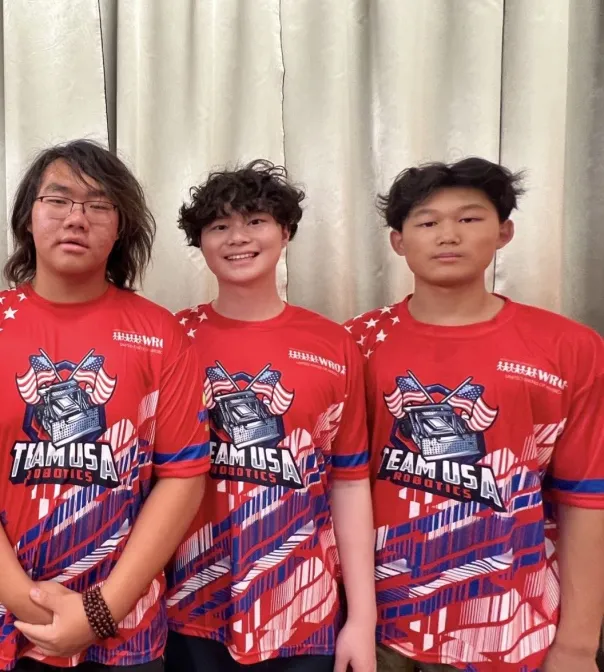
\includegraphics[width=7cm]{teamPhoto.png}
           \caption{From left to right: Yangxuezhe Sun, Jiarui Hu, William Wu}
           \label{fig:enter-label}
       \end{figure}

    \vspace{1cm}
            \section*{Team Members and Roles}
\subsection{William Wu}
A 10th-grade student passionate about coding from Rancho Cucamonga High School, William oversaw the development and integration of AI algorithms. He ensured the AI system adapted to different track conditions and optimized the vehicle's performance in real time. His expertise in machine learning was instrumental in debugging and troubleshooting technical issues. Throughout the project he was the primary proponent of the GitHub developement and created elaborate diagrams and 3D models for the group. By applying complex AI models, William played a crucial role in uniting the team and ensuring cohesive and efficient work throughout the project.

\subsection{Yangxuezhe (Harry) Sun}
A 11th-grade student with experience in programming and structural design from Rancho Cucamonga High School, Yangxuezhe assembled the physical vehicle and coded the algorithms enabling autonomous operation. His work focused on precise implementation of Pulse Width Modulation (PWM) for motor control, ensuring fine adjustments to the vehicle’s steering and speed. His work on the hardware part of the solution greatly helped put the project in motion and marked the start of the development of AI models.

\subsection{Jiarui (Jerry) Hu}
A 12th-grade student from Western Christian High School with extensive knowledge of artificial intelligence and 3D modeling, Jiarui was responsible for optimizing the AI system for real-time decision-making processes and editing videos for the team. He also helped organize the GitHub while maintaining a crucial role in supporting the team and making sure everythign was functioning.

\subsection{Coach Fei Guo}
As a seasoned mentor with a background in autonomous systems, Coach Fei Guo provided invaluable guidance. He helped refine AI models and hardware integration while fostering critical and creative problem-solving skills within the team.
        
\section*{Technical Solution Design}
Our vehicle’s design represents a careful combination of mechanical engineering, AI development, and control system integration, with a strong emphasis on robust, modular, and Self-Designed hardware. The platform for the vehicle is an RC car (Bezgar Remote Control Car), chosen for its durability, speed, and reliability in high-performance environments. This base provided a sturdy foundation for handling the demanding tasks of the WRO competition. \par

\begin{figure}[H]
            \centering
            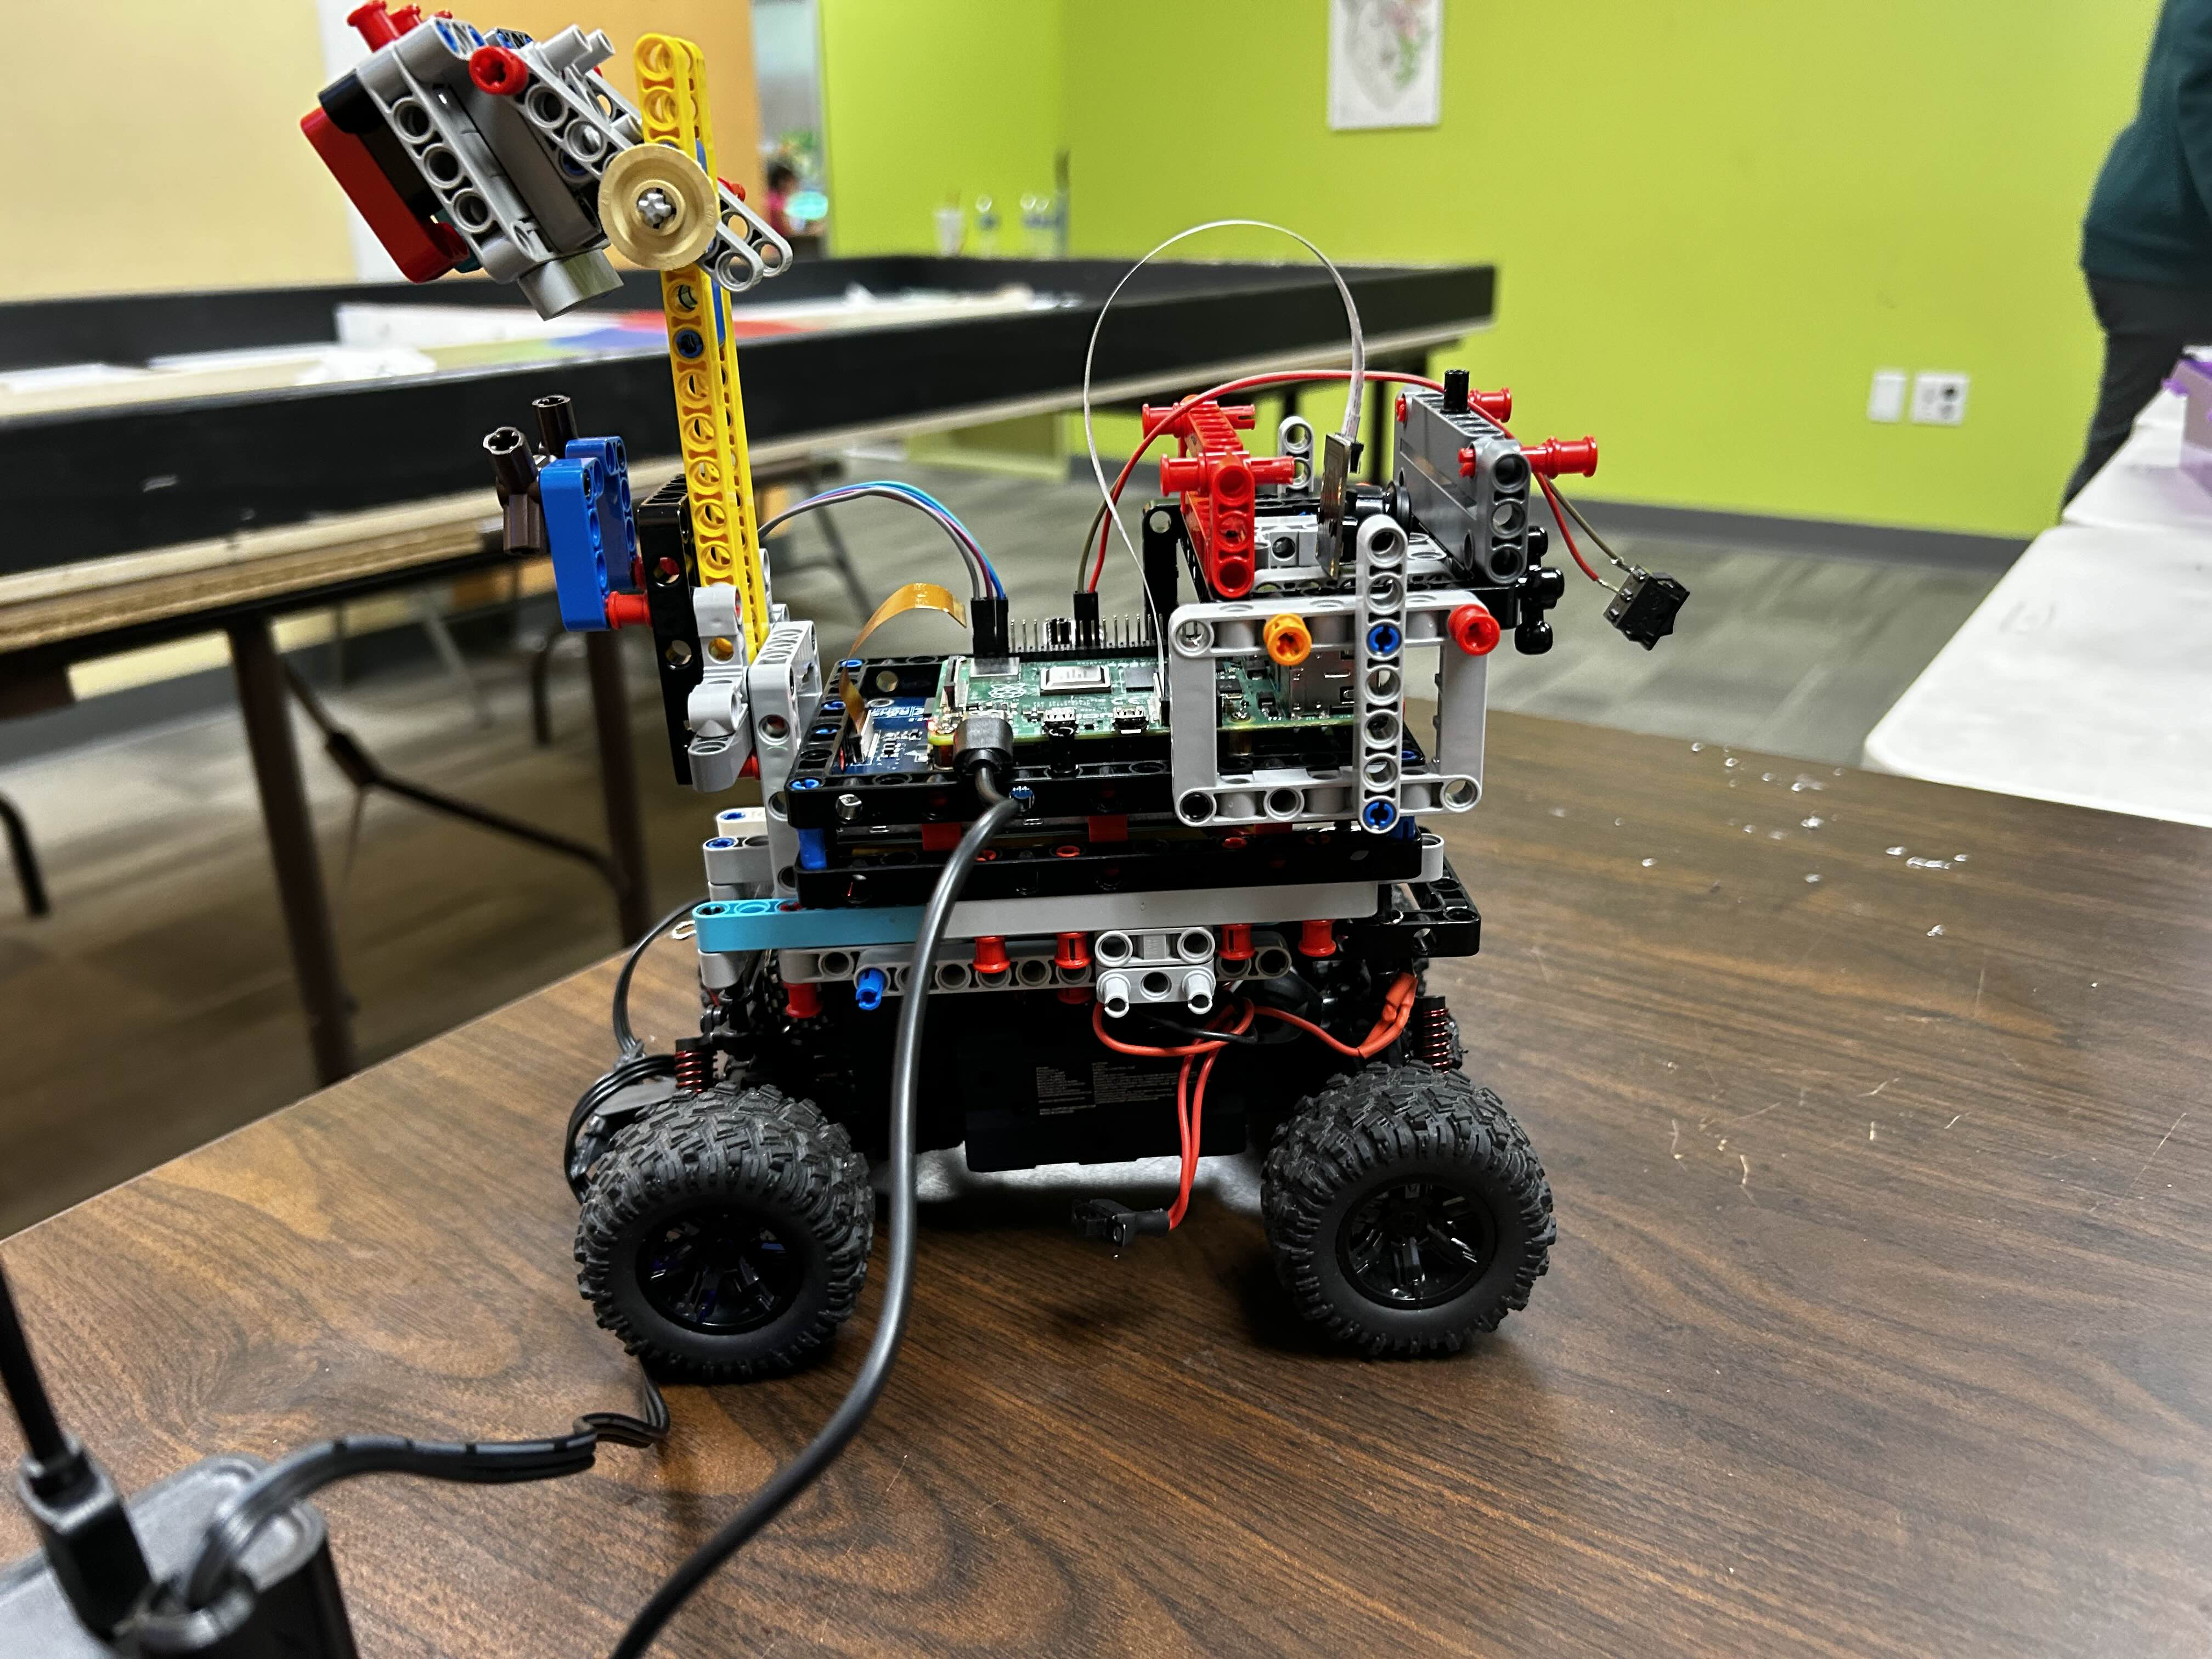
\includegraphics[width=7cm]{carleft.jpg}
            \caption*{Our vehicle solution}
        \end{figure}

We designed a modular LEGO structure mounted atop the RC car to securely house the essential hardware components. The LEGO construction was chosen for its adaptability and standardization of parts, allowing us to make iterative adjustments during testing phases. This modularity proved critical when fine-tuning the positioning of the camera, gyroscope, and Raspberry Pi, ensuring optimal performance across varied track conditions and lighting environments.


At the heart of the vehicle lies the Raspberry Pi 4 Model B, which served as the central processing unit (CPU). It processes data from the camera and gyroscope in real time, running AI models to make instantaneous decisions. The Raspberry Pi was selected for its computational power, compact size, and support for advanced machine learning frameworks such as TensorFlow. Most of the code is located on the raspberry pi inside a hard drive (SD card) and is able to accessed easily

\begin{figure}[H]
            \centering
            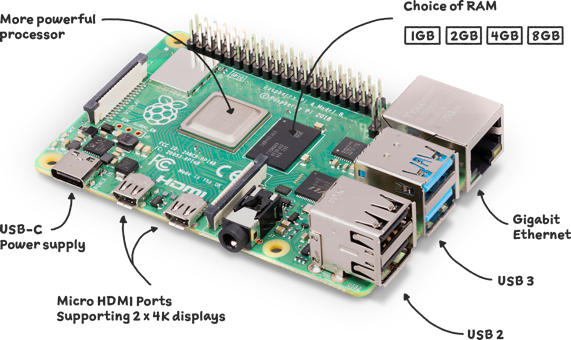
\includegraphics[width=7cm]{raspberry-pi-4-labelled-f5e5dcdf6a34223235f83261fa42d1e8.png}
            \caption*{Raspberry Pi computing system}
        \end{figure}

The vehicle is equipped with a Raspberry Pi Camera Module v2, which provides a live video feed of the track. This feed is critical for the AI system to recognize track boundaries, detect obstacles, and make informed navigational decisions. The camera was mounted on an adjustable LEGO arm, enabling precise positioning.

The WT901 gyroscope was integrated into the system to monitor the vehicle’s orientation and angular velocity. This sensor played a key role in determining when to stop the vehicle after 3 laps and monitored orientation data throughout the run.

To achieve precise control over the vehicle’s movements, we implemented Pulse Width Modulation (PWM with ic2 interface) for motor management. PWM allowed fine-tuned adjustments to the vehicle's speed and steering. This control system was essential for the raspberry pi to assimilate with the RC car and control it. Additionally, PWM optimized power consumption, ensuring reliable performance throughout extended competition runs.

To improve performance, the stock RC car tires were replaced with high-traction, off-road tires. These upgraded tires provided enhanced stability and grip on track surface and allowed it to make sharp turns without accidentally drifting off-course.

By integrating these carefully selected hardware components into a cohesive design, our vehicle was able to handle the rigorous challenges of the WRO competition, demonstrating exceptional adaptability and performance in real-world scenarios.


    \newpage

\section{Software and Functionality of Codes}

The software system for our autonomous vehicle is stored on an SD card within the Raspberry Pi. It consists of multiple Python scripts, each designed to handle specific tasks in the development, testing, and execution of the AI models. Below is a detailed breakdown of these code files:

\begin{enumerate}
    \item manage.py is the main code that collects training data for the AI model

    \begin{figure}[H]
            \centering         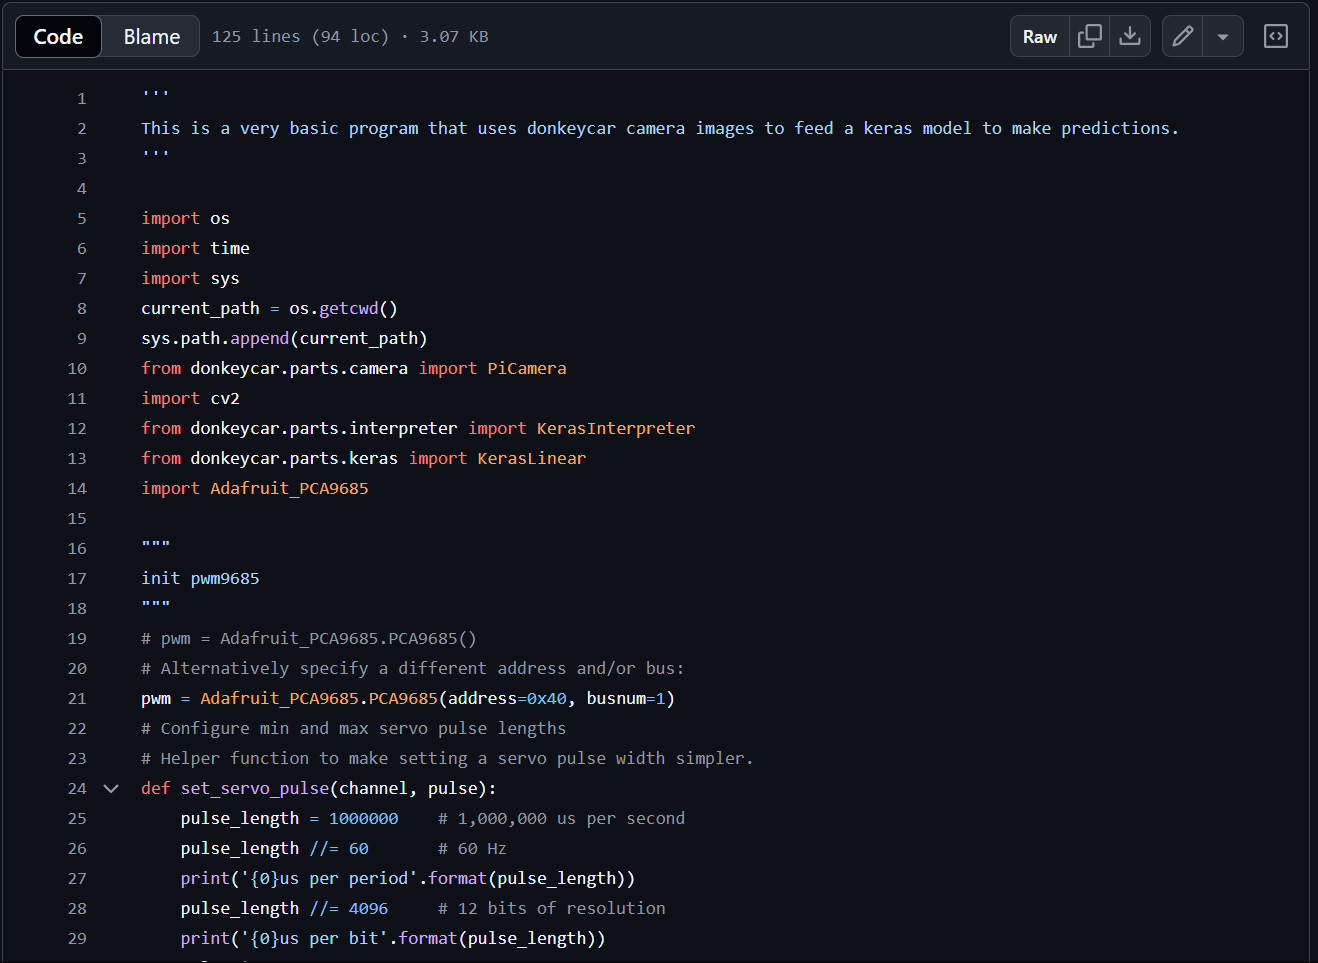
\includegraphics[width=8cm]{manage.py.png}
            \caption*{Code for manage.py}
    \end{figure}

    \item config.py defines the default Pulse Width Modulation (PWM) values, which are critical for controlling the vehicle's motors and steering. These parameters ensure consistent and precise vehicle movement.
    \item calibrate.py is used to synchronize the AI model with the vehicle’s hardware, this script ensures that sensor data and system responses are accurately aligned during operation.
    \item airc\_drive10.py serves as a testing tool for the AI model. It allows us to evaluate and debug the vehicle's performance in a controlled environment before deploying it in competition.
    \item myconfig.py provides the foundational framework upon which we built our customized AI solutions which is imported form the donkey car forums.
    \item main\_freerun.py is the final AI program for the freerun segment of the competition. This script enables the vehicle to autonomously complete three laps around the track and stop precisely based on gyroscope readings.
    \item main\_obstacle.py is the final AI program for the obstacle run segment of the competition. It drives the car through two laps while dynamically avoiding obstacles according to the competition rules. The program then performs an additional lap (clockwise or counterclockwise as specified by the rules) and concludes with a final lap, parking the vehicle accurately in the designated slot.
\end{enumerate}

These scripts seamlessly integrate with the electromechanical systems, including the Raspberry Pi, gyroscope, camera, and motors. Together, the software and hardware ensure a smooth and efficient training process, real-time decision-making, and flawless execution during competition. This harmonious interaction between software and hardware underscores the sophistication of our autonomous vehicle’s design.

\section{AI Training Process}
The AI model for our autonomous vehicle was developed using real-world data collected during manual driving sessions on the competition track, facilitated by the script manage.py. These sessions enabled us to capture critical data, including camera images and vehicle control inputs, which served as the foundation for training the model.

\begin{figure}[H]
    \centering         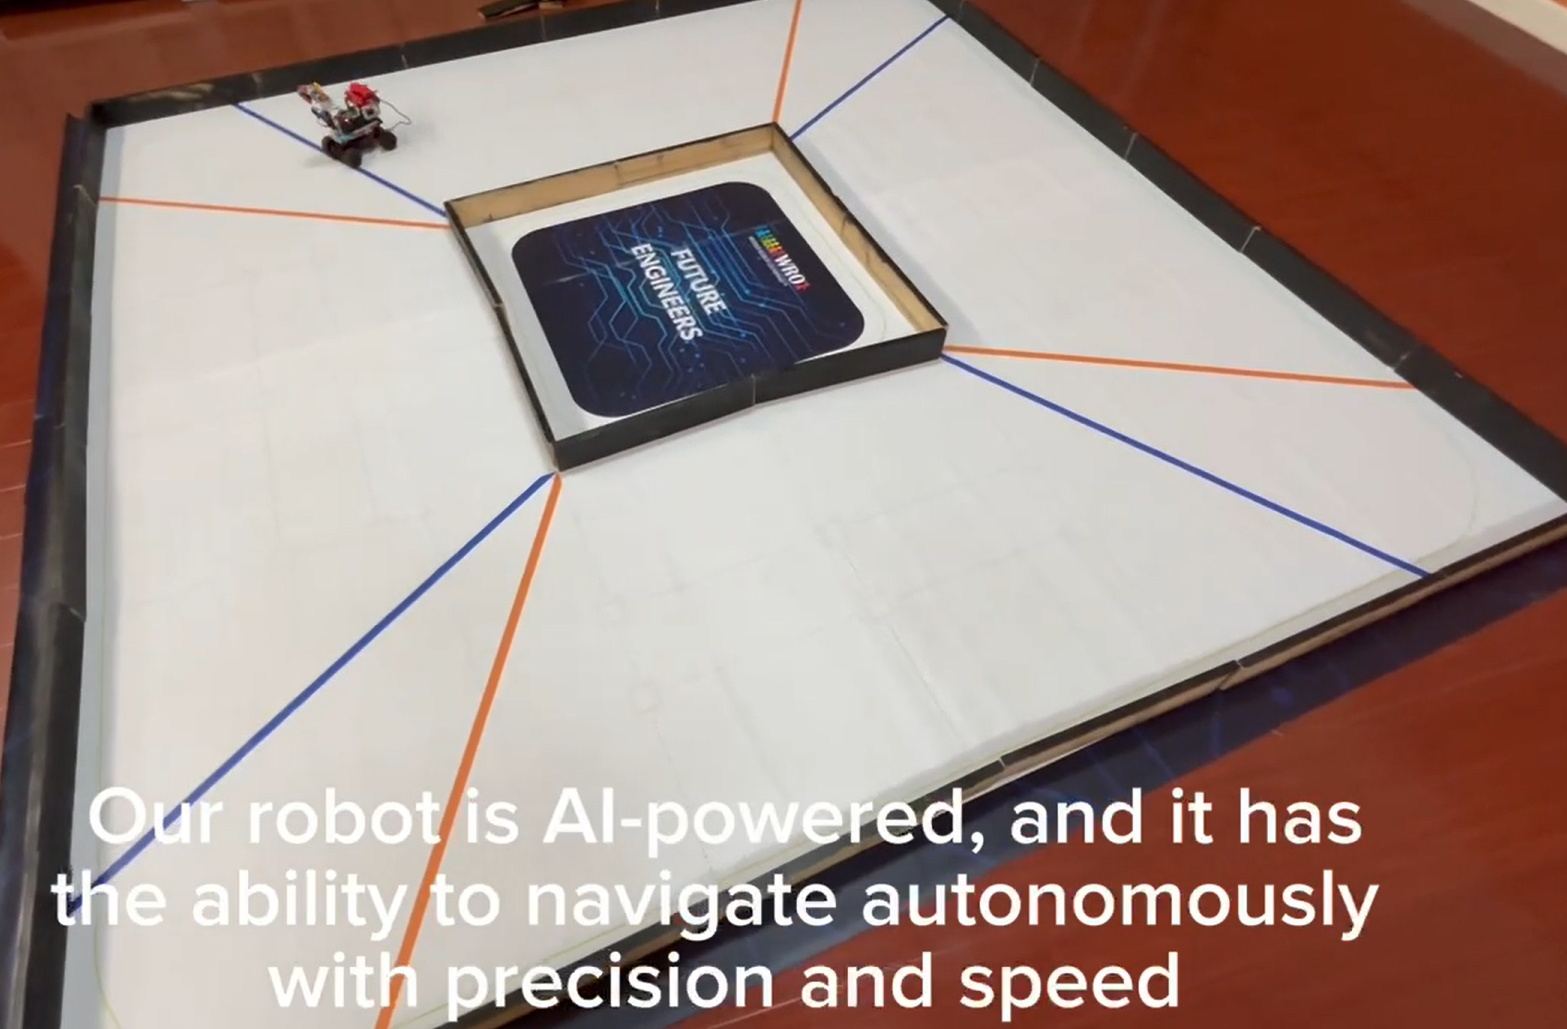
\includegraphics[width=8cm]{training.png}
    \caption*{Data Collection Process for Vehicle}
\end{figure}

To process this data, we used FileZilla to transfer the training datasets from the Raspberry Pi to our development computers. Once the data was prepared, we leveraged TensorFlow within a Miniconda3 command prompt environment to build and train a Convolutional Neural Network (CNN). The CNN was specifically designed to analyze visual inputs from the vehicle’s camera and map them to precise throttle and steering commands, enabling the AI to learn how to navigate the track effectively.

\begin{figure}[H]
    \centering         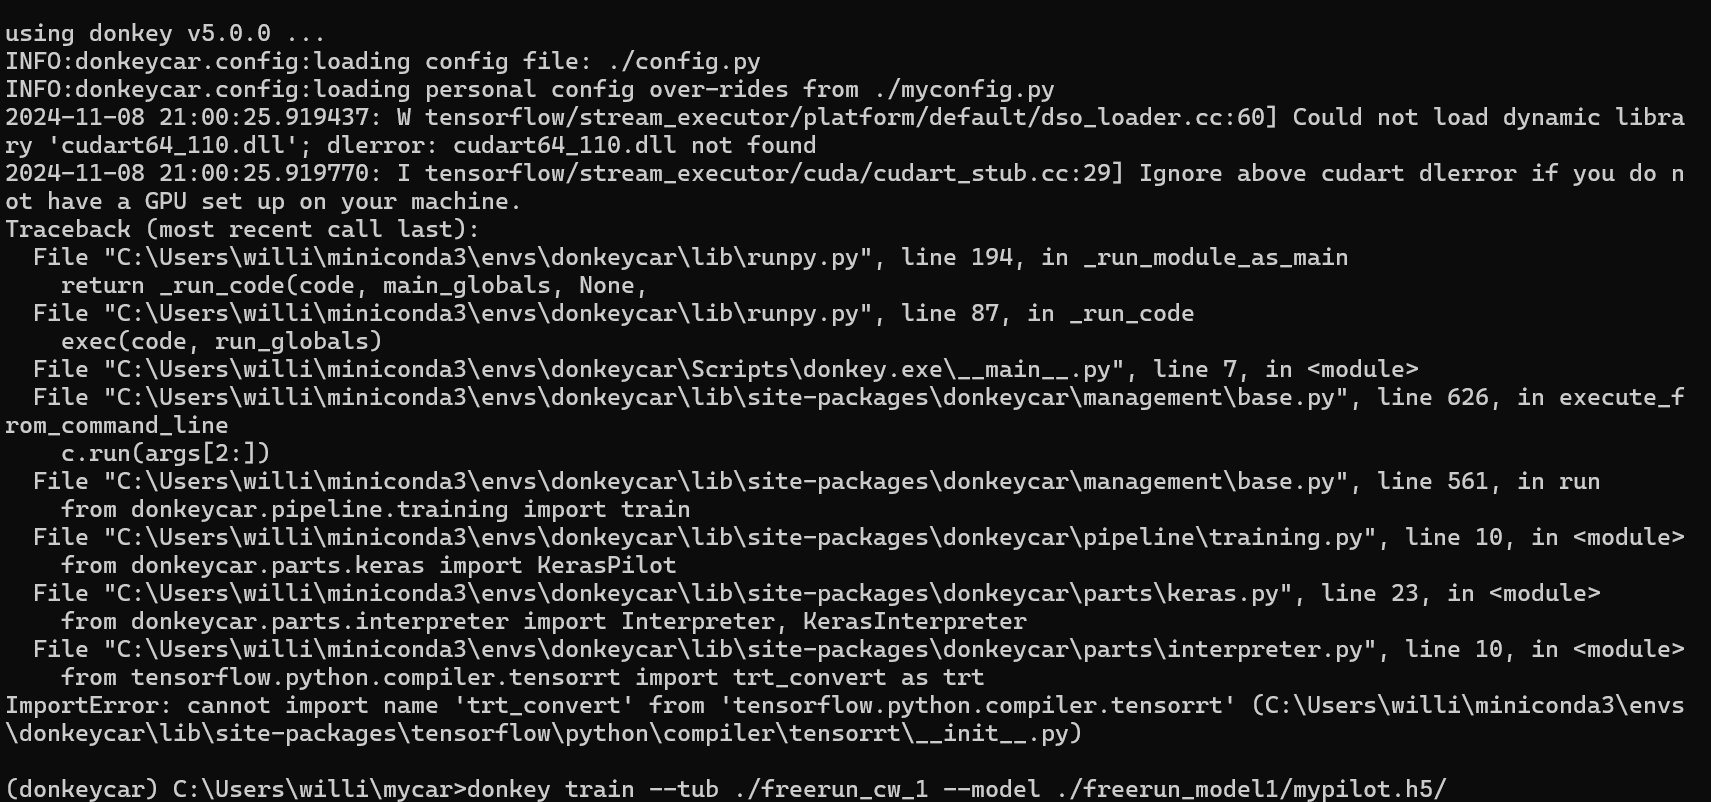
\includegraphics[width=8cm]{miniconda.png}
    \caption*{Training Process using Miniconda3}
\end{figure}

The training process was iterative, involving extensive testing and fine-tuning to optimize the model's accuracy and performance. After each iteration, we evaluated the AI's ability to handle various track scenarios, including straight paths, sharp turns, and obstacle navigation. With each improvement, the AI system became increasingly adept at interpreting visual inputs, making real-time decisions, and autonomously navigating the complex track conditions with precision.

\section{Power and Sense Management}

Effective power management was essential to ensure reliable performance throughout the competition. To achieve this, Pulse Width Modulation (PWM) was employed to optimize the vehicle's power consumption, allowing us to extend battery life while maintaining consistent operation and precision control.

Our vehicle was powered by two sources:

\begin{enumerate}
    \item Li-Polymer Model 603048 (7.4V, 850mAh): This battery powered the RC car's motors, ensuring sufficient energy for movement and steering.

    \item HYD001 Portable Charger: This device powered the Raspberry Pi, which in turn supplied energy to the gyroscope and camera.

    \begin{figure}[H]
    \centering         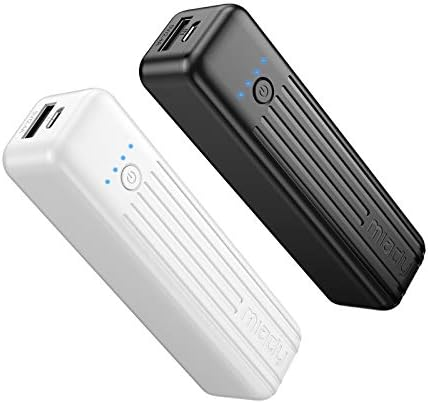
\includegraphics[width=8cm]{battery2.jpg}
\end{figure}
    
\end{enumerate}

This power setup was carefully designed to ensure stability and reliability during operation. The modular structure allowed for efficient energy distribution across all components, providing sufficient power for extended competition runs and maintaining the system’s overall functionality.

\section{Model Management}
Once the AI model has been trained, it is uploaded back to the Raspberry Pi using FileZilla and stored in a designated folder named airc\_drive. This streamlined process ensures that the model is readily accessible for deployment.

\begin{figure}[H]
    \centering         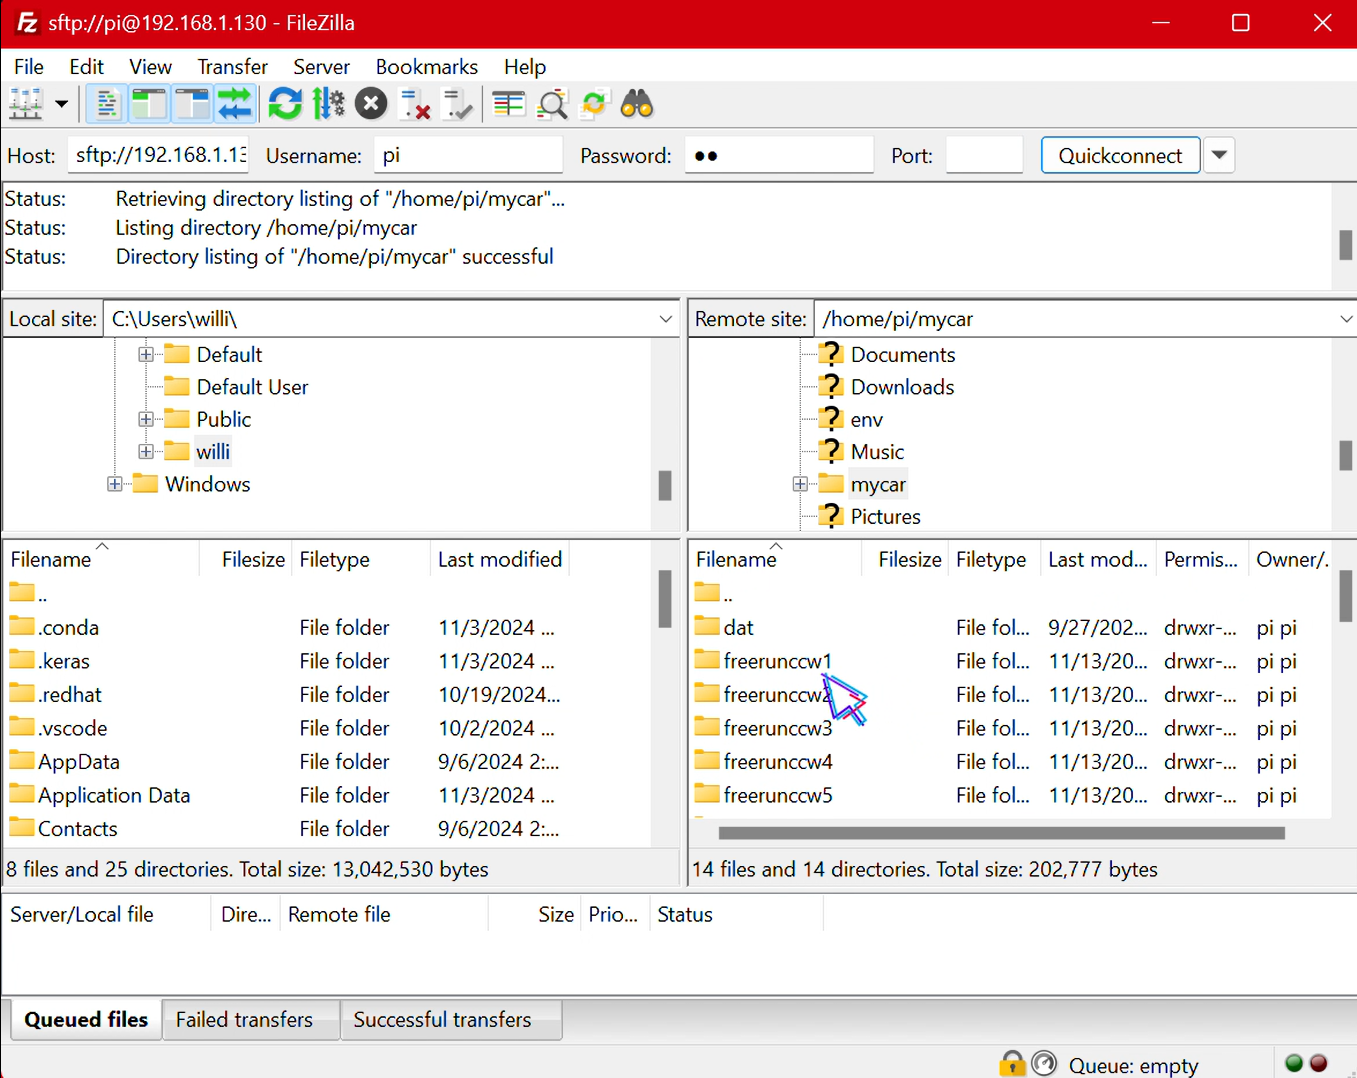
\includegraphics[width=8cm]{filezilla.png}
    \caption*{Transferring the Model Back to the Raspberry Pi}
\end{figure}

\newpage

The trained model can be executed using airc\_drive10.py, serving as the foundation for both the main\_freerun.py and main\_obstacle.py. These scripts allow the model to autonomously control the vehicle, performing tasks such as navigating the freerun course or completing obstacle avoidance and parking challenges.

This robust model management system guarantees smooth integration, ensuring the AI functions reliably and enables the successful completion of all project objectives.

\section{Conclusion}

Our project represents the culmination of months of dedication, innovation, and teamwork in designing and developing a truly autonomous vehicle. By combining advanced AI techniques, robust hardware design, and seamless integration of mechanical and electrical components, we created a system capable of navigating complex environments, overcoming challenges, and completing the 2024 WRO Future Engineers competition without human intervention.

Through this journey, we deepened our understanding of critical concepts in machine learning, control systems, and robotics while honing our problem-solving and collaboration skills. From building the physical structure and integrating sensors to training and deploying the AI model, each phase of the project brought unique challenges and opportunities for growth.

This experience not only prepared us for the rigors of the competition but also inspired us to envision the broader applications of autonomous systems in real-world scenarios. We are proud to have contributed to the evolving field of robotics and autonomous vehicles, and we look forward to exploring even more ambitious projects in the future. We welcome everyone to use the models and projects in the GitHub to expand on the growing progress in the AI vehicle industry and succeed in their own competition!

\begin{itemize}
    \item Github Link: https://github.com/Utcassyxz/USA-Future-Engineers---DriverUS/tree/main
    \item Youtube Link: https://www.youtube.com/@DriverUS-future-engineers
\end{itemize}

    \end{multicols}
\end{document}
